\section{Aproksymacja sygnału}
    Aproksymacją sygnału $x(t)$ jest:
    \begin{equation*}
        x(t) \approx \sum_{n=1}^{N}a_nb_n(t)
    \end{equation*}
    czyli:
    \begin{align*}
        x(t)  \textbf{+}e(t) = \sum_{n=1}^{N}a_n\cdot b_n(t)\\
        x(t) = \sum_{n=1}^{N}a_n\cdot b_n-e(t)
    \end{align*}
    gdzie współczynniki $a$ i $b$ odpowiadają macierzom:
    \begin{equation*}
        b = A \cdot a\\
    \end{equation*}
    \begin{align*}
        % 
        b = \left[\begin{array}{c}
            x\circ b_1\\
            x\circ b_2\\
            x\circ b_3\\
            ...\\
            x\circ b_N
        \end{array}\right] &&
        A = \left[\begin{array}{c c c c}
            b_1\circ b_1 & b_2\circ b_1 & ... & b_N\circ b_1\\
            b_1\circ b_2 & b_2\circ b_2 & ... & b_N\circ b_2\\
            b_1\circ b_3 & b_2\circ b_3 & ... & b_N\circ b_3\\
            ...          & ...          & ... & ...\\
            b_1\circ b_N & b_2\circ b_N & ... & b_N\circ b_N
        \end{array}\right] &&
        a = \left[\begin{array}{c}
            a_1\\
            a_2\\
            a_3\\
            ...\\
            a_N
        \end{array}\right]
    \end{align*}

    W gdyby wektory byłyby ortogonalne, całość sprowadza się do prostego równania:
    \begin{align*}
        a_k = \frac{x\circ b_k}{||b_k||^2} && k = 1, 2, ..., N
    \end{align*}

    Kiedy nasze wektory są znormalizowane to:
    \begin{align*}
        ||b_k||^2 = 1\\
        a_k = x\circ b_k  && k = 1, 2, ..., N
    \end{align*}
    
\newpage
\section{Baza Harra (ortonormalna)}
    \begin{align*}
        H_{0,0}(t) = \Pi(t-0.5) && D: t\in <0, 1>\\
        H_{0,1} = \Pi(2\cdot (t-0.25))-\Pi(2\cdot(t-0.75))\\
        H_{k,m} = 2^{\frac{k}{2}}\cdot H(2^k\cdot (t-\frac{m-1}{2^k})) && m = 1, 2, ..., 2^k
    \end{align*}

    \begin{multicols}{2}
        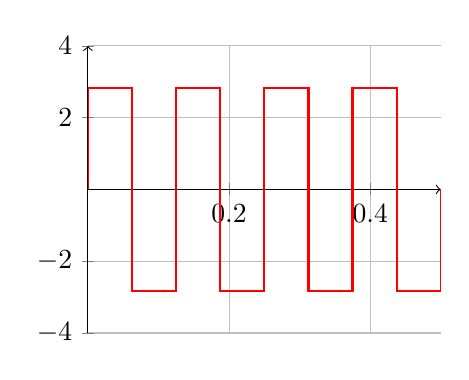
\begin{tikzpicture}
            \begin{axis}[
                width =0.5\textwidth,
                xmajorgrids = true,
                ymajorgrids = true,
                legend style={at={(0.85, 0.25)},anchor=north,legend cell align=south east},
                axis lines=middle,
                axis line style={->},
                xmax = 0.5,
                ymin = 0,
                ymax = 4,
                ymin = -4
            ]
                \addplot[red, thick, mark=none, const plot] coordinates 
                {(0,0) (0, 2.82) (0.0625,2.82) (0.0625, -2.82) (0.125, -2.82) (0.125, 2.82) (0.1875, 2.82) (0.1875, -2.82) (0.25, -2.82) (0.25, 2.82) (0.3125, 2.82) (0.3125, -2.82) (0.375, -2.82) (0.375, 2.82) (0.4375, 2.82) (0.4375, -2.82) (0.5, -2.82) (0.5, 0)};
            \end{axis}
        \end{tikzpicture}

        Czyli kolejne sygnały bazy:
        \begin{gather*}
            b_1(t) = H_{0,0}(t)\\
            b_2(t) = H_{1,\sum}(t)\\
            b_3(t) = H_{2,\sum}(t)\\
            b_4(t) = H_{3,\sum}(t)\\
            ...
        \end{gather*}
    \end{multicols}

\section{Baza Walsha}
    \begin{align*}
        W_{0, 0}(t) = \Pi(t-0.5) && D: t\in<0, 1>\\
        W_{0, 1}(t) = W_{0, 0}(2t)+(-1)^1\cdot W_{0, 0}(2\cdot(t-0.5))\\\\
        W_{k, 2m-1}(t) = W_{k-1, m}(2t)+(-1)^{m-1}\cdot W_{k-1, m}(2\cdot(t-0.5)) && dla\ k > 1\\
        W_{k, 2m}(t)   = W_{k-1, m}(2t)+(-1)^{m}  \cdot W_{k-1, m}(2\cdot(t-0.5)) && dla\ k > 1
    \end{align*}

    \begin{multicols}{2}
        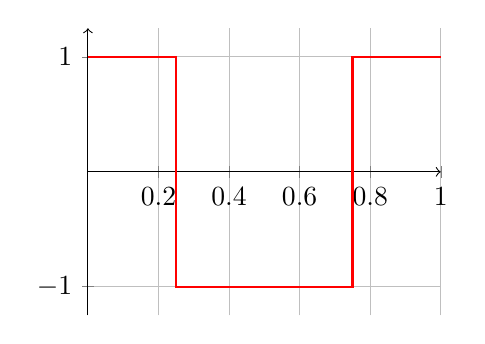
\begin{tikzpicture}
            \begin{axis}[
                width =0.5\textwidth,
                xmajorgrids = true,
                ymajorgrids = true,
                legend style={at={(0.85, 0.25)},anchor=north,legend cell align=south east},
                axis lines=middle,
                axis line style={->},
                xmax = 1,
                ymin = 0,
                ymax = 1.25,
                ymin = -1.25
            ]
                \addplot[red, thick, mark=none, const plot] coordinates 
                {(0, 1) (0.25, 1) (0.25, -1) (0.75, -1) (0.75, 1) (1, 1)};
            \end{axis}
        \end{tikzpicture}
        
        Analogicznie jak w bazie Harra
    \end{multicols}